\documentclass[12pt,a4paper]{article}
\usepackage[utf8]{inputenc}
\usepackage[spanish]{babel}
\usepackage{graphicx}
\usepackage{hyperref}
\usepackage{xcolor}

\title{Manual de Usuario - Administrador de Mapas}
\author{TUS DATOS AQUÍ}
\date{FECHA}

\begin{document}

\maketitle
\tableofcontents
\newpage

\section{Introducción}
El \textbf{Catastro Metropolitano} es una plataforma web interactiva diseñada para la gestión y visualización de mapas catastrales urbanos. Permite a los usuarios diseñar, editar y guardar la geometría de calles, avenidas, curvas viales y cuadras en tiempo real. 

Esta herramienta está pensada para agilizar el trabajo de los urbanistas y administradores locales, ofreciendo una experiencia visual fluida. Puedes acceder al panel de administración directamente desde el siguiente enlace:
\href{https://mapas-api.pages.dev/}{Acceder al Panel Frontend}

\section{Acceso y Vista Principal}
Al ingresar al enlace, te encontrarás con la vista principal de la aplicación. Desde aquí, puedes explorar los mapas disponibles o crear un entorno de trabajo desde cero. La interfaz ha sido diseñada priorizando la claridad y la facilidad de uso.

\begin{figure}[h]
    \centering
    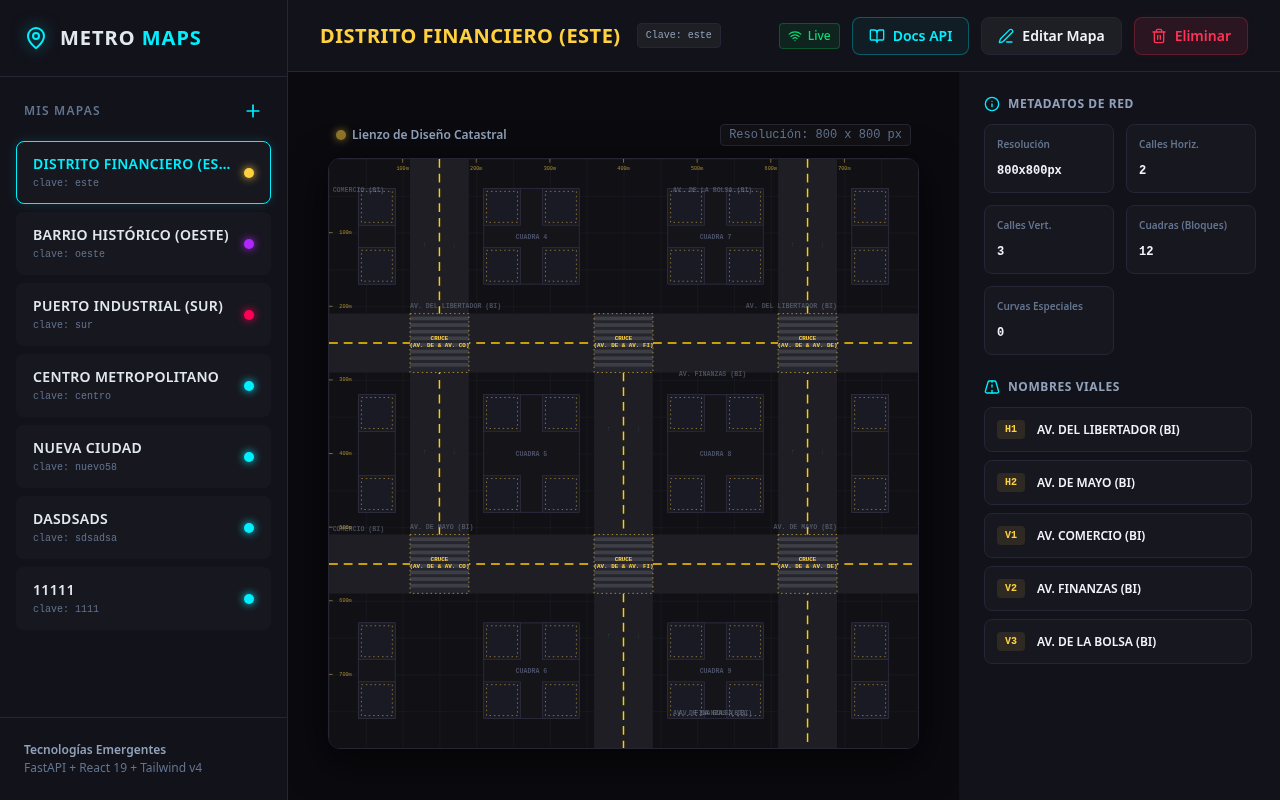
\includegraphics[width=1\textwidth]{../docs_assets/frontend.png}
    \caption{Pantalla principal del frontend (Alojado en Cloudflare Pages)}
\end{figure}

\section{Exploración y Edición de Mapas}
El sistema te permite buscar mapas específicos por su \textbf{Clave}, que actúa como el identificador único del mapa en la base de datos.

\subsection{Cargando un Mapa Existente}
\begin{enumerate}
    \item Ubica la barra de búsqueda en la interfaz superior.
    \item Ingresa la clave del mapa que deseas editar, por ejemplo: \texttt{sur} o \texttt{centro}.
    \item Presiona enter. El mapa se cargará en el lienzo (canvas) principal, mostrando sus avenidas, cuadras y distribución geométrica actual.
\end{enumerate}

\subsection{Panel de Herramientas de Dibujo}
Una vez que el mapa esté cargado, el panel lateral te permitirá interactuar con el lienzo:
\begin{itemize}
    \item \textbf{Dibujar Calles y Avenidas}: Selecciona la herramienta de vía y haz clic en el lienzo para trazar nuevas vías de circulación. Puedes ajustar el grosor para diferenciar calles secundarias de avenidas principales.
    \item \textbf{Crear Curvas Viales}: Utiliza los puntos de control Bézier para ajustar el diseño urbano de las esquinas, rotondas y retornos.
    \item \textbf{Definir Cuadras}: Selecciona la herramienta de polígonos para delimitar zonas residenciales, comerciales o parques.
\end{itemize}

\subsection{Mejores Prácticas de Edición}
\begin{itemize}
    \item \textbf{Precisión:} Haz zoom en el canvas para ajustar los vértices de las cuadras con mayor precisión.
    \item \textbf{Colores Tiemáticos:} Asigna colores temáticos coherentes para diferenciar zonas comerciales de zonas residenciales.
\end{itemize}

\section{Guardado y Tiempo Real}
Todos los cambios que realices usando las herramientas de edición se comunican automáticamente al servidor central (Supabase).
\begin{itemize}
    \item \textbf{Autoguardado:} No es necesario recargar la página ni pulsar un botón de guardar; cada trazo se sincroniza en milisegundos.
    \item \textbf{Colaboración:} El sistema cuenta con \textbf{sincronización en tiempo real}, por lo que si otro operador está viendo el mismo mapa desde otro dispositivo, verá tus trazos y modificaciones aparecer instantáneamente en su pantalla.
\end{itemize}

\section{Guía de Uso para Consumidores de la API}
Si eres un integrador o desarrollador que necesita consumir los datos de los mapas desde otro sistema, debes interactuar directamente con nuestro Backend.

\subsection{Acceso a la Documentación (Swagger)}
Ingresa a: \href{https://tecnologia-atkj.onrender.com/api/docs}{https://tecnologia-atkj.onrender.com/api/docs}.
Aquí encontrarás la definición completa de cada endpoint.

\subsection{Paso a paso para crear un mapa vía API}
\begin{enumerate}
    \item Expande el endpoint \texttt{POST /api/mapas}.
    \item Haz clic en el botón \textbf{"Try it out"}.
    \item En el campo \texttt{Request body}, introduce un JSON válido con la estructura del mapa, especificando la \texttt{clave}, el \texttt{nombre} y las dimensiones (\texttt{width}, \texttt{height}).
    \item Haz clic en \textbf{"Execute"}. 
    \item Si vas al Frontend y buscas la clave que acabas de crear, verás el lienzo en blanco listo para que los operadores comiencen a dibujar usando la configuración inicial que inyectaste vía API.
\end{enumerate}

\end{document}
